\subsection{Temperatur}\label{subsec:Temperatur}
Um einen Einblick in das Temperaturverhalten des Motors zu erlangen, wird im nächsten Versuch die Erwärmung in Abhängigkeit der Drehzahl bei konstantem Moment gemessen. Die Messung erfolgt bei einer Drehzahl von 1550 RPM und bei 2550 RPM und einem jeweiligen Drehmoment von 32Nm. Die Starttemperatur des Motors ist jeweils ca. 60°C und ist solange betrieben worden, bis er eine Betriebstemperatur von 100°C erreicht. Die Versuchsresultate in der Abbildung \ref{fig:Temperatur} wurde ohne zusätzliche Ventilation des Motors durchgeführt. Alle Versuche wurden gemäss den Bedingungen in Tabelle \ref{tab:Temperatur} durchgeführt.



\begin{table}[H]
	\centering
	\begin{tabular}{C{4cm} C{4cm} C{3cm}} 
		\multicolumn{3}{c}{\textbf{Versuchsbedingungen}} \\
		{Messgrösse}& {Bedingung} & {Wert}\\ \hline\hline 
		Spannung (DC)   & konstant &   96 V     \\
		Strom (DC)   & vernachlässigt &   -     \\
		Leistung (AC)   & vernachlässigt &   -    \\
		Drehzahl   & konstant &   1500/2500 RPM    \\
		Drehmoment-Sollwert   & konstant &   32 Nm    \\
		Motor-Temperatur   & gemessen &   40-100 °C    \\
		Controller-Temperatur   & gemessen &   35-64 °C    \\
	\end{tabular}
	\caption{Versuchsbedingungen Temperatur}\label{tab:Temperatur}
\end{table}

\begin{figure}[H]
	\centering
	\includegraphics[width=0.8\linewidth]{Temperatur.jpg}
	\caption{Erwärmung}\label{fig:Temperatur}
\end{figure}


Da die Leistung sowohl vom Drehmoment als auch von der Drehzahl abhängt, wird  der Motor beim Versuch mit 2550 RPM mit einer erhöhten Leistung betrieben, wodurch auch ein grössere Strom fliesst. Aus diesem Grund ist die Erwärmung des Motors bei höheren Drehzahlen dementsprechend schneller. In Abbildung \ref{fig:TemperaturMotor} und \ref{fig:TemperaturController} ist der Temperaturverlauf des Motors bzw. des Controllers ersichtlich. Beim Motor ist die Messung zuerst mit nur einem zusätzlichen Ventilator (Anordnung hinter Motor) gemessen und anschliessend mit drei zusätzlichen Ventilatoren (Anordnung hinter und beidseitig des Motors) durchgeführt worden. Beim Controller sind ebenfalls zwei Messungen mit unterschiedlicher Kühlung durchgeführt. Die eine Messung mit einem grossen thermischen Kühlkörper (hier diente der Messtisch als Kühlkörper), die andere ohne Kühlkörper (mit thermischer Isolation zum Messtisch). Bei diesen Versuche wurde auch die Zeit zum Abkühlen gemessen, während die Drehzahl konstant bei 2500 RPM blieb.


\begin{figure}[H]
	\centering
	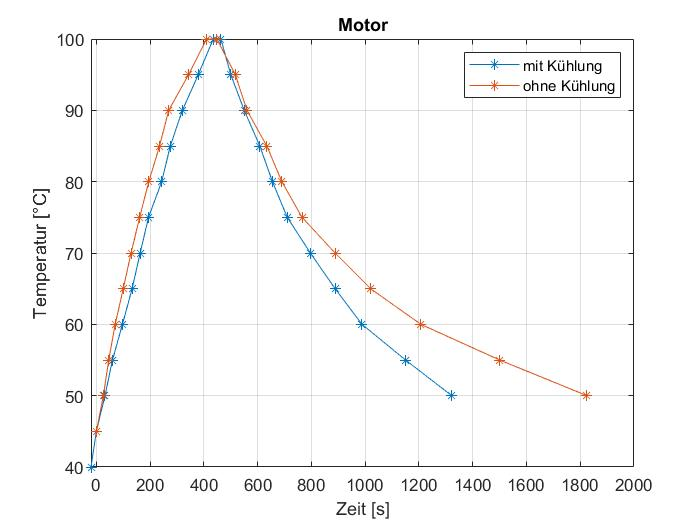
\includegraphics[width=1.0\linewidth]{TemperaturMotor.jpg}
	\caption{Temperaturverlauf Motor}\label{fig:TemperaturMotor}
\end{figure}

In der Temperaturkurve des Motors ist zu erkennen, dass die Zeit zum Abkühlen bedeutend grösser ist, als die der Erwärmung bei Nennmoment. Weil der Motor im Abrollbetrieb mit einem hohen Wiederholungsintervall (Kapitel \ref{sec:Hardware}) betrieben werden kann, muss der Motor zusätzlich gekühlt werden. Dasselbe Verhalten ist auch beim Controller in Abbildung \ref{fig:TemperaturController} ersichtlich.

\begin{figure}[H]
	\centering
	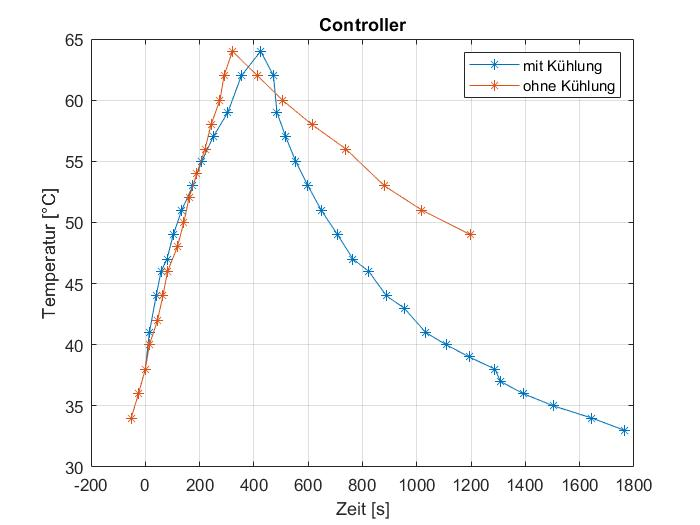
\includegraphics[width=0.8\linewidth]{TemperaturController.jpg}
	\caption{Temperaturverlauf Controller}\label{fig:TemperaturController}
\end{figure}

Es ist deutlich erkennbar, dass der Controller ohne Kühlung viel langsamer abkühlt. Der Hersteller weist im Datenblatt\cite{ControllerUserGuide} jedoch keine max. Temperatur aus, weswegen wir eine Temperaturobergrenze von 65°C annehmen.